\documentclass{standalone}
\usepackage{tikz}
% create a new adjust box
\usepackage{tikzscale}
\usepackage{lscape}
\usepackage{tikz}
% use to adjust the positionS
\usetikzlibrary{positioning}
\usetikzlibrary{calc}
\tikzset{abs1/.style={xshift=3cm,yshift=2cm}}
\usetikzlibrary{shapes.geometric,arrows}
\tikzstyle{arrow}=
[thick,<-,>=stealth]

\begin{document}
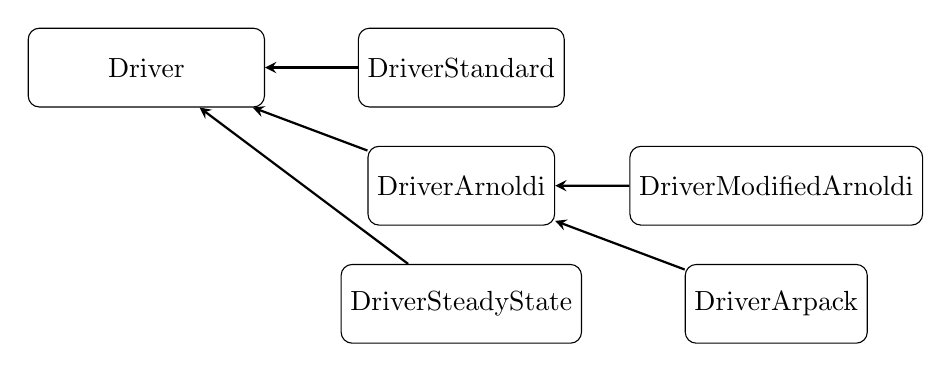
\begin{tikzpicture}[scale=0.2,node distance=2cm]
    \node (A)
    [rectangle,
    rounded corners,
    minimum width=3cm,
    minimum height=1cm,
    text centered,
    draw=black]
    {Driver};
    \node (B)
    [rectangle,
    rounded corners,
    minimum width=1cm,
    minimum height=1cm,
    text centered,
    draw=black,
    right of=A,
    xshift=2cm,
    yshift=0cm]
    {DriverStandard};
    \draw[arrow](A)--(B);
    \node (B)
    [rectangle,
    rounded corners,
    minimum width=1cm,
    minimum height=1cm,
    text centered,
    draw=black,
    right of=A,
    xshift=2cm,
    yshift=-1.5cm]
    {DriverArnoldi};
    \draw[arrow](A)--(B);
    \node (C)
    [rectangle,
    rounded corners,
    minimum width=1cm,
    minimum height=1cm,
    text centered,
    draw=black,
    right of=B,
    xshift=2cm,
    yshift=0cm]
    {DriverModifiedArnoldi};
    \draw[arrow](B)--(C);
    \node (C)
    [rectangle,
    rounded corners,
    minimum width=1cm,
    minimum height=1cm,
    text centered,
    draw=black,
    right of=B,
    xshift=2cm,
    yshift=-1.5cm]
    {DriverArpack};
    \draw[arrow](B)--(C);
    \node (B)
    [rectangle,
    rounded corners,
    minimum width=1cm,
    minimum height=1cm,
    text centered,
    draw=black,
    right of=A,
    xshift=2cm,
    yshift=-3cm]
    {DriverSteadyState};
    \draw[arrow](A)--(B);
\end{tikzpicture}
\end{document}